\chapter{Zadanie 5}
Kolejnym krokiem było stworzenie prostego graficznego panelu operatora,
przy pomocy oprogramowania \texttt{GT Designer}. Składa się on z tytułu,
oraz sześciu słupków, gdzie każdy reprezentuje poziom innego sygnału.
Każdy ze słupków jest podpisany, tak, aby było wiadomo jaki sygnał reprezentuje.
Wygląd panelu przedstawia rysunek \ref{pic:panel}.
Ułożenie owych słupków nie było szczególnie planowane i należałoby je jakoś
rozsądnie posortować, na przykład zestawiająć trzy parametry każdego sygnału
obok siebie. Należałoby również podać wartości liczbowe sygnału pod każdym ze
słupków. Biorąc pod uwagę, iż jest to jedynie wersja poglądowa, nie przywiązywaliśmy
do tego zbyt dużej wagi, jednak jesteśmy świadomi usprawnień jakie należy
dokonać, gdyby taki system faktycznie miał być użytkowany.

\begin{figure}[tb]
  \centering
  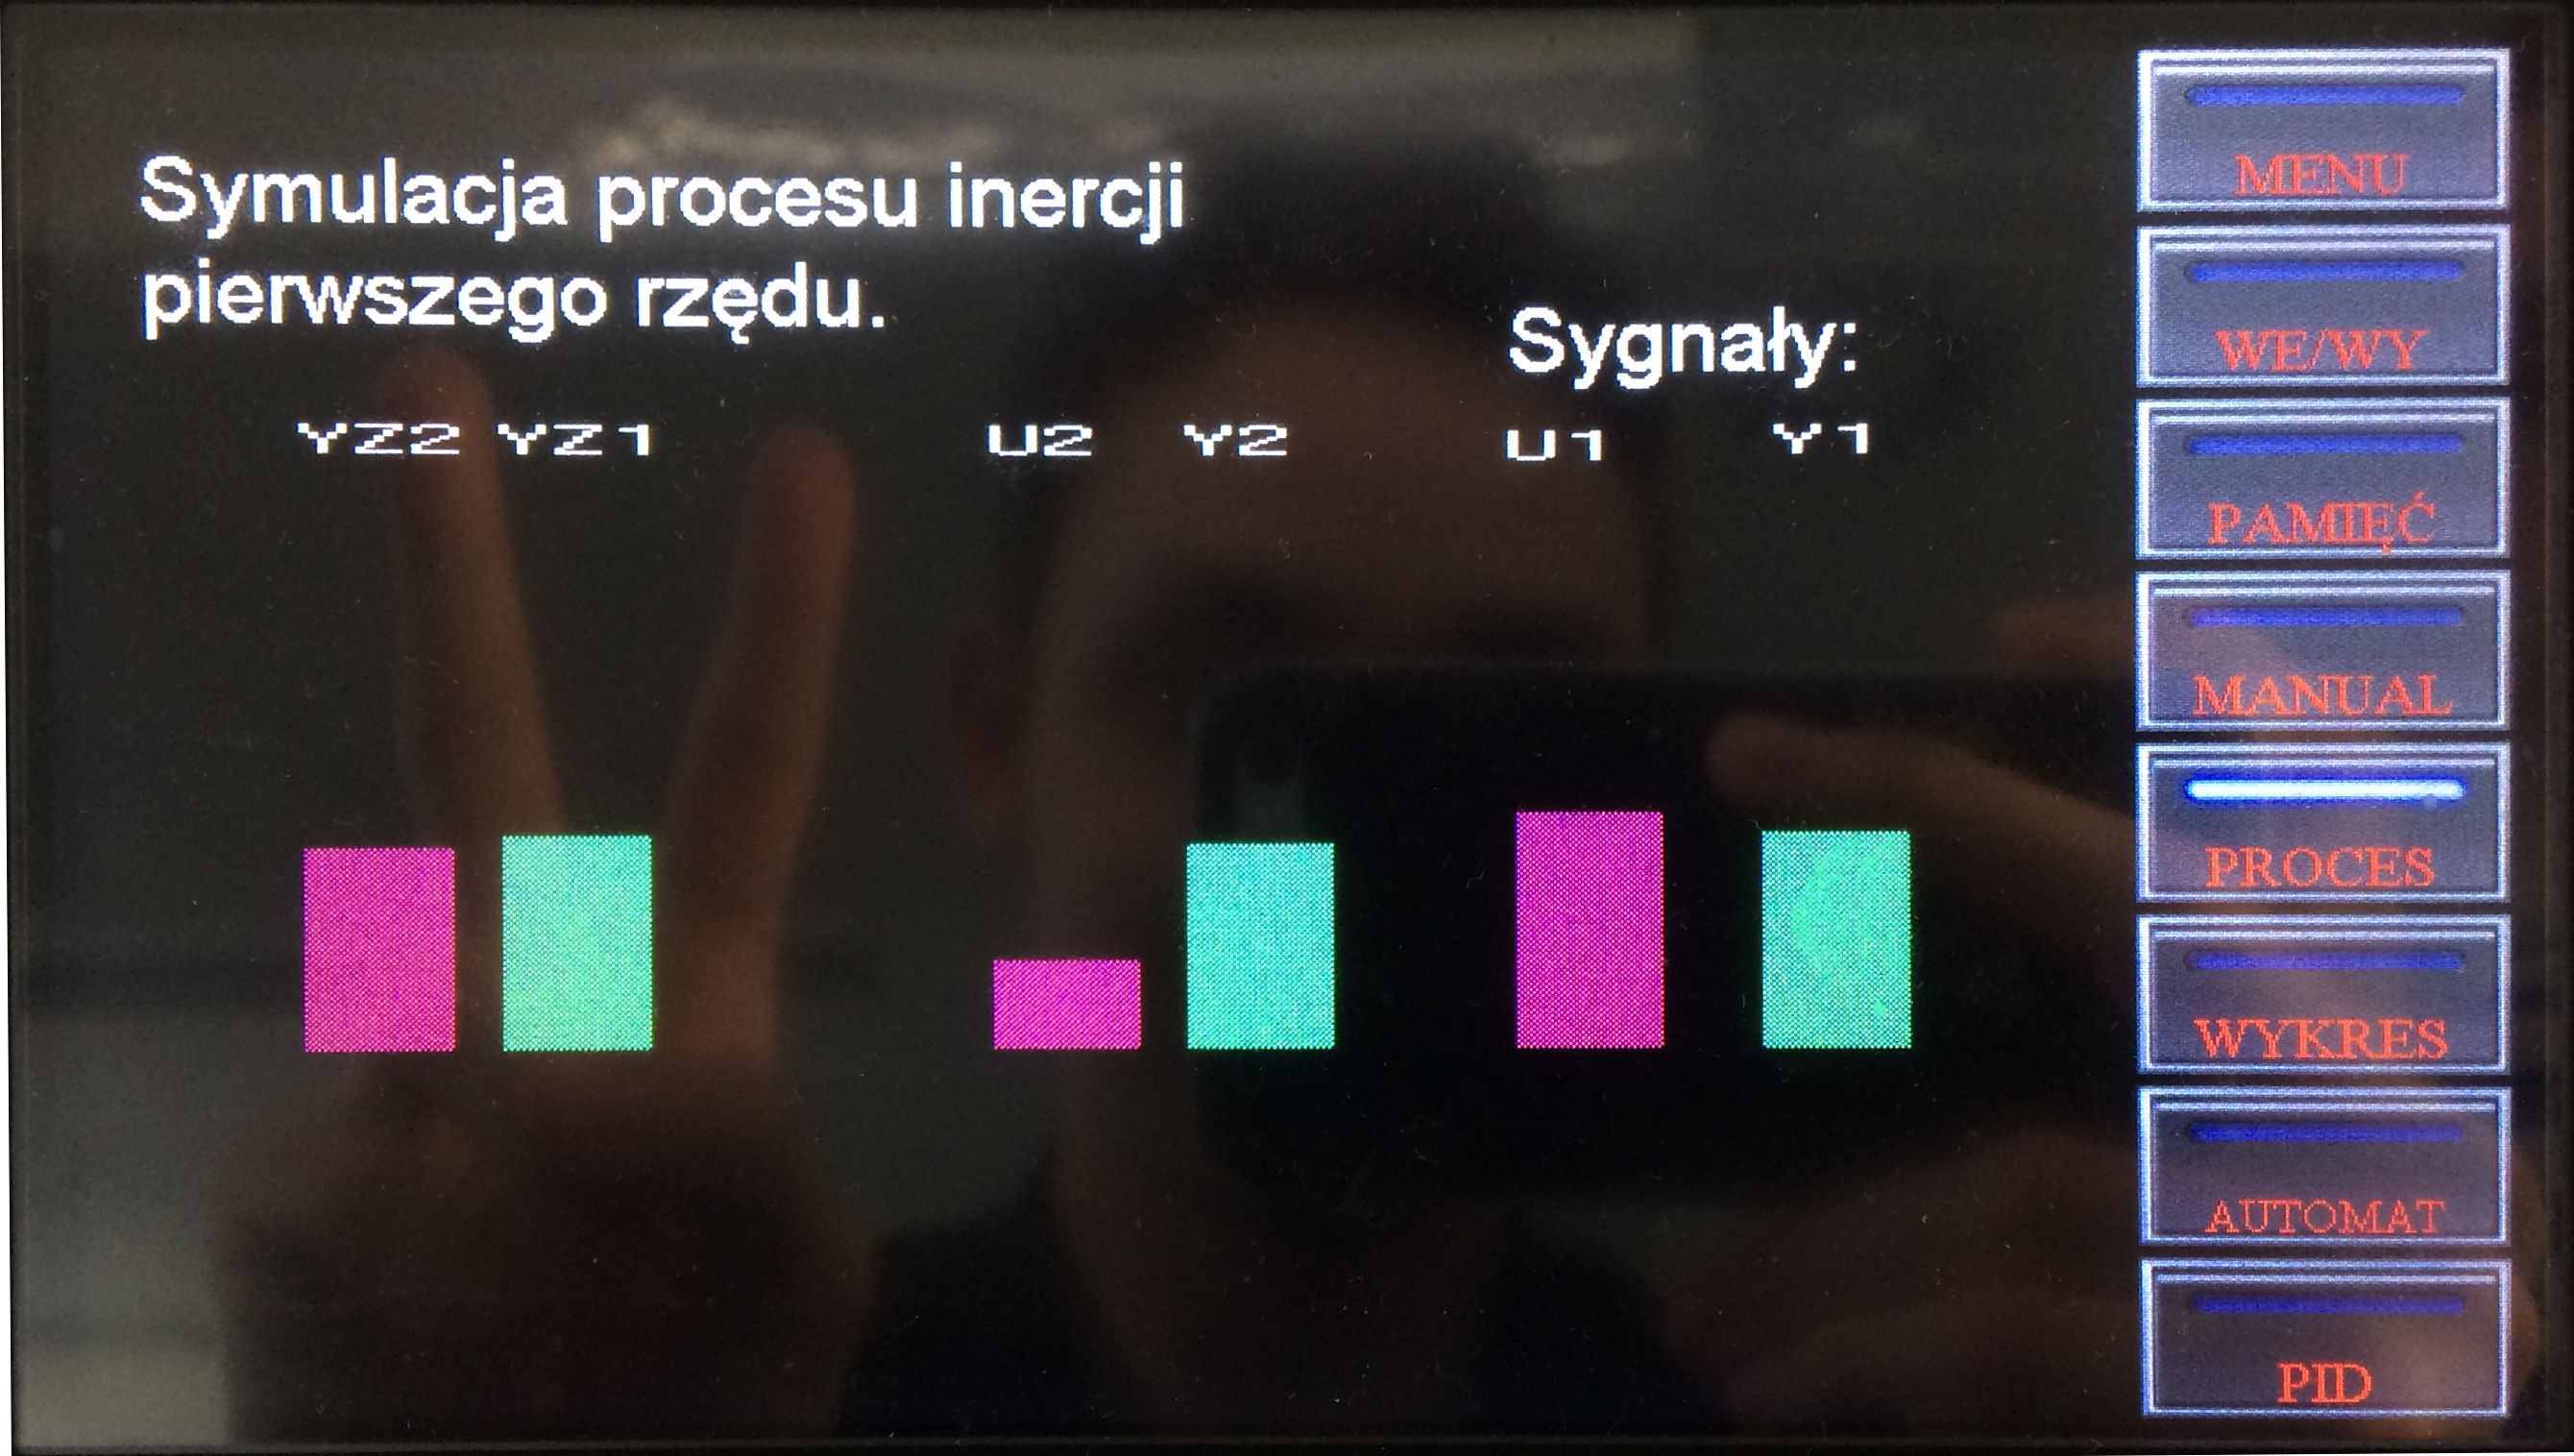
\includegraphics[width=0.9\textwidth]{Pictures/proces.jpg}
  \caption{Panel operatora}
  \label{pic:panel}
\end{figure}
